% 2017 KTS
% 텍 매크로 파일 만들기

\documentclass{beamer}

\usefonttheme[onlymath]{serif}
\usetheme{metropolis}
\metroset{outer/progressbar=head}

\usepackage{fancyvrb}
\usepackage{kotex}
\hypersetup{pdfencoding=auto}

\def\TEX/{$\textrm{\TeX}$}
\def\LATEX/{$\textrm{\LaTeX}$}

% title
\title{텍 매크로 파일 만들기}
\subtitle{플레인 텍으로 만드는 레시피 카드}
\date{2017년 2월 11일 토요일}
\author{남수진}
\institute{
  2017 한국텍학회 학술대회 및 정기총회 \\
  동국대학교 법학관 B253호}
\titlegraphic{\hfill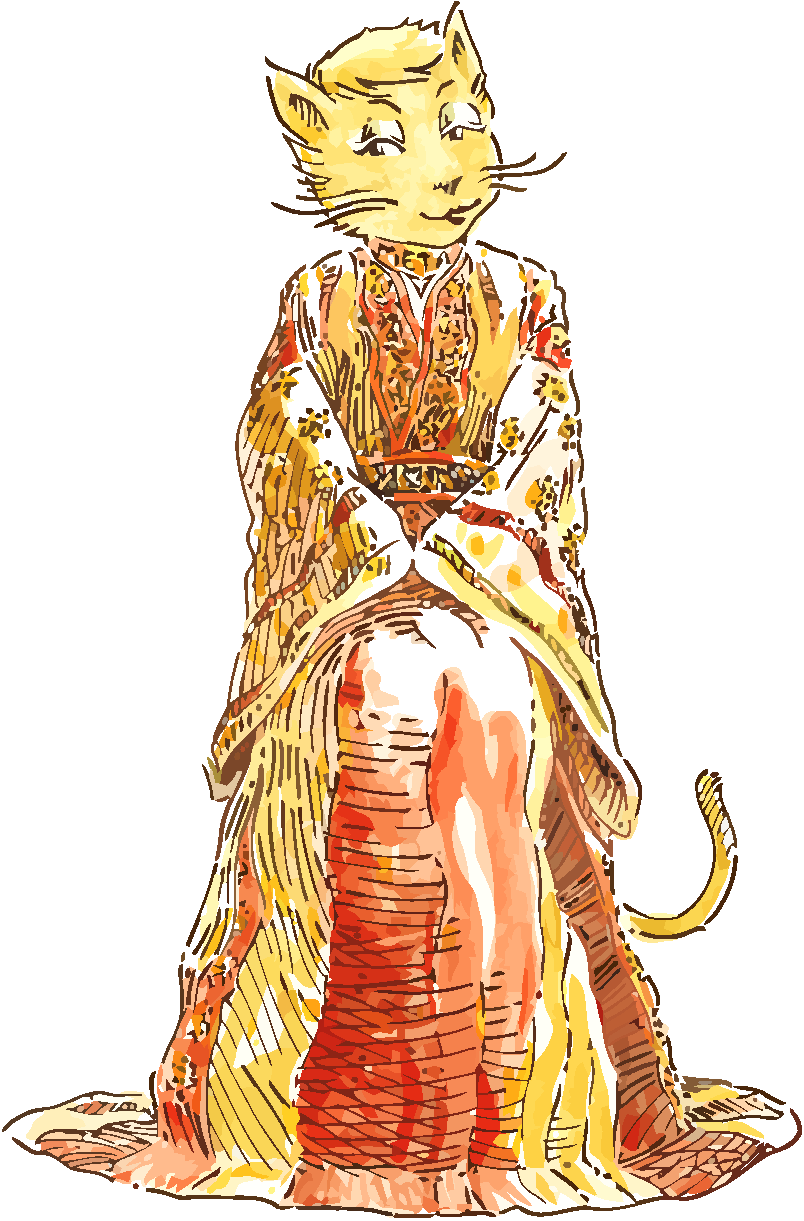
\includegraphics[height=3cm]{meta.pdf}}


%%
\begin{document}

\maketitle

%
\begin{frame}[standout]
  왜 플레인 텍인가?
\end{frame}


%
\begin{frame}[fragile]{플레인 텍 Plain \TEX/}
  \begin{itemize}
  \item 도널드 크누스가 만든 텍 시스템, \alert{``virgin'' \TEX/}
    \begin{itemize}
    \item 매크로가 하나도 없는 갓난 아이 같은 텍. 순수 그 자체
    \item 문서 작성에 사용하기에는 무리가 있다.
    \end{itemize}
  \item 순수 텍을 실제로 사용할 수 있도록 기본적인 세팅과 편리한 매크로들을 제공한다.
  \item ``텍 포멧 파일은 이렇게 만드는 것이다.'' 라는 표본 제시
  \end{itemize}
\end{frame}


%
\begin{frame}[fragile]{라텍 \LATEX/}
  \begin{itemize}
  \item 우리가 흔히 문서 작성할 때 텍이라고 부르는 것
  \item 고품질의 조판을 위한 문서 작성 시스템
  \item 어느 정도 분량이 있는 구조를 갖춘 문서 작성에 제격이다.
  \item 클래스 파일, 다수의 패키지 파일과 복잡한(?) 글꼴 세팅이 필요하다.
  \end{itemize}
  
  \begin{Verbatim}[fontsize=\small]
    \documentclass[a4paper,tocentry,microtype]{oblivoir}
    \usepackage[dbl4x6]{fapapersize}
    \usepackage[dvipdfmx]{graphicx}
    \usepackage{hyperref}
    \usepackage{wrapfig}
    \usepackage{caption}
    ...
  \end{Verbatim}
\end{frame}


%
\begin{frame}{1995년 TUG 미팅에서}
  Questions and Answers with Prof. Donald E. Knuth, 
  TUGboat \textbf{17} (1996), 7--22
  \begin{description}
  \item[Silvio Levy:] How come you don't use \LATEX/? [\textsl{laughter}]
  \item[Don:] How come I don't use \LATEX/? [\textsl{laughter}]
    I'm scared of \alert{large systems!} [\textsl{louder laughter\/}]
    Bart?
  \end{description}
\end{frame}


%
\begin{frame}{플레인 텍을 사용하면}
  \begin{itemize}
  \item 매년 새롭게 나오는 텍라이브를 설치할 필요가 없다.
  \item 심심할 때마다 {\small\alert{\texttt{tlmgr update --all --self}}}를
    칠 필요가 없다.
  \item 20년 전에 만들었던 텍 문서가 여전히 잘 컴파일 된다.
  \item 프리엠블로 고민할 필요가 없다. 폰트에 대한 욕심을 줄이면, 할 일이 아무것도 없다.
  \item 한글 문서라면, {\small\alert{\texttt{\string\input\ kotex.sty}}}
    한줄로 끝.
  \item {\scriptsize 자신만의 간단한 매크로를 만들어야 할 때가 있다.}
  \end{itemize}
  
  구조적이지 않고 일정한 틀이 없는 간단한 문서 작성에는 플레인 텍을 사용해 보자.
\end{frame}


%
\begin{frame}[standout]
  레시피 카드 매크로
\end{frame}


%
\begin{frame}[fragile]{Active 문자}
  \begin{itemize}
  \item 백슬래시 없이도 명령어 역할을 하는 문자
  \item 플레인 텍에서는 \alert{\string~}
  \item 주로 \texttt{\string\let}을 이용하여 명령어로 동작한다.
  \end{itemize}
  \begin{Verbatim}
    \catcode`\*=13 \let*=\medskip
  \end{Verbatim}
\end{frame}


%
\begin{frame}[fragile]{\texttt{\string\obeylines}}
  \begin{itemize}
  \item 텍은 엔터(CR)도 간격을 나타내는 문자로 인식한다. (\verb+^^M+)% ascii 참고
  \item 엔터를 우리가 기대하는 기능 그대로! 
  \end{itemize}

  \begin{table}[ht]
  \begin{minipage}[t]{.4\textwidth}
  \begin{Verbatim}[fontsize=\small]
{\obeylines
Roses are red,
\quad Violets are blue;
Rhymes can be typeset
\quad With boxes and glue.
\smallskip}
  \end{Verbatim}
  \end{minipage}%
  \qquad\qquad
  \begin{minipage}[t]{.4\linewidth}
    {\obeylines
      Roses are red,
      \quad Violets are blue;
      Rhymes can be typeset
      \quad With boxes and glue.
      \smallskip}
  \end{minipage}
  \end{table}
  
  \begin{Verbatim}
   \def\obeylines{\catcode`\^^M=13 \let^^M=\par}
  \end{Verbatim}
\end{frame}


%
\begin{frame}{참고 문서}
  \begin{itemize}
  \item \href{http://ftp.ktug.org/tex-archive/systems/knuth/dist/tex/}
    {The \TeX book}
  \item \href{https://tug.org/TUGboat/tb17-1/tb50knut.pdf}
    {TUG95, Questions and Answers with Prof. Donald E. Knuth}
  \item \href{https://www.tug.org/TUGboat/tb08-3/tb19knut.pdf}
    {Macros for Jill}
  \item \href{https://github.com/sjnam/TeX}
    {github.com/sjnam/TeX}

  \end{itemize}
\end{frame}


%
\begin{frame}[standout]
  감사합니다
\end{frame}

\end{document}

